\chapter{Background}
\label{chapter:background} 


This chapter examines how autism manifests in children, how it affects their communication skills, and what assistive sign language is. This chapter also examines what research has already been done with social robots as communication therapy tools for autistic children, and social robots as teachers of sign language. At the end of this chapter, this knowledge is synthesized into five design guidelines, which will guide the design process of the robot in chapter \ref{chapter:design}.


%%%%%%%%%%
%%%%%%%%%%


\section{Autism in children}


Autism or autism spectrum disorder (ASD) is a developmental disorder which is characterized by impaired social behavior, impaired communication and language, and a narrow range of interests and activities that are unique to the individual and carried out repetitively \cite{WHOautism}.  The intervention described in this thesis is targeted at improving impaired communication.

In 2017, the World Health Organization reported that worldwide, 1 in 160 children has an autism spectrum disorder \cite{WHOautism}. According to a Danish study, ASD diagnoses have been increasing, with incidence rates rising from 9.0 to 38.6 per 100 000 people from 1995 to 2010 in Denmark. Increases were most pronounced among adolescents, adults and females \cite{jensen2014time}. Diagnoses of ASD are also increasing globally. This apparent increase could be due to improved awareness, expansion of diagnostic criteria, or better diagnostic tools and improved reporting \cite{WHOautism}.

ASD begins in childhood, and in most cases the condition is apparent during the first five years of a child's life. Autism usually persists into adolescence and adulthood. The level of functioning among individuals with ASD is highly variable, and ability ranges from profound cognitive impairment to superior performance in certain areas \cite{WHOautism}. Research has shown that the level of functioning of adults with ASDs depends on how well they were using language before school age \cite{tetzchner}.

Early interventions targeted at improving the speech, communication or behavior of the autist are aimed at improving quality of life, rather than curing the disorder. When provided early enough, interventions can improve the person's self-care, communication and social skills \cite{tetzchner}. Due to this, the intervention introduced in this thesis focuses on children.

%%%%%%%%%%
%%%%%%%%%%

\subsection[Communication and language difficulty as a characteristic of autism spectrum disorder]{Communication and language difficulty as a \\characteristic of autism spectrum disorder}

50 \% of children with autism remain functionally mute in adulthood \cite{puheSuomi, peeters1999autism}. For those that do learn to speak, the development of language is often delayed, and the level of language is highly variable \cite{puheSuomi}.

According to the current understanding, the key problem of autism is a lack of ``Theory of Mind'', which means that people with autism have trouble recognizing that other humans have thoughts and feelings, and have trouble anticipating others' behavior \cite{baron1985does, frith2003autism}. People with autism also experience problems in integrating pieces of information into a coherent whole. These core problems contribute to the problems of communication, social interaction and flexibility that people with ASDs experience \cite{frith2003autism}. Problems experienced in social interactions discourage autistic people even further from making an effort, which in turn minimizes opportunities to learn communication and social skills, creating a negative feedback loop \cite{autismi}.

To avoid this loop, teaching autistic children communication and social skills needs to be clear and structured so as not to confuse and distress the person even further. Therapy for children with ASDs often focuses on teaching basic social skills such as eye contact, turn taking, joint attention and emotion recognition \cite{autismi}. Because problems in speech can be anticipated, therapy for people with autism often includes practicing using other forms of communication, such as using assistive sign language, gestures, picture symbols or photos \cite{puheSuomi, tincani2004comparing}. These forms of communication can be used either as alternative communication, which replaces speech, or augmentative communication, which supports speech \cite{puheSuomi}. In the intervention presented in this thesis, the focus is specifically on assistive sign language, which is a form of augmentative communication.


%%%%%%%%%%
%%%%%%%%%%

\subsection{Assistive sign language as a communication method for people with autism spectrum disorder}

Signing is the most used form of both alternative and augmentative communication used in Finland \cite{puheSuomi} and globally \cite{tetzchner}. Signing can hasten the acquisition of speech for some autistic individuals, since during signing, visual and motoric memory support the auditory memory used for speech \cite{bonvillian1981sign, autismi}. Early sign language teaching has been shown to advance the development of children, especially their language, cognitive and social skills \cite{puheSuomi}. 

Assistive sign language, which is a form of augmentative communication, is used simultaneously with speech, in support of it. Individual signs are borrowed from Finnish sign language, but the grammar and structural rules associated with Finnish sign language are not used. The most important words of sentences are signed simultaneously as the words are spoken \cite{puheSuomi}. According to speech therapist Lehtonen, who works with autistic children, the most important word is determined by the context. For example, when saying ``Let's go to the kitchen to eat.'', the most important word can be ``kitchen'' if eating is usually done somewhere else, or it could be ``eat'' if eating is being done at an exceptional time, and the kitchen is usually reserved for other activities  (A. Lehtonen, personal communication, June 25, 2018).

Finnish sign language signs are constructed of four components: hand shape, placement, movement and orientation. In addition to hands, facial expressions and body posture are also used to communicate signs. Mouth shape can also be used to communicate \cite{puheSuomi}. According to speech therapist Lehtonen, the hands are most important in assistive signing. Facial expressions can be used to communicate the tone of the statement. For example, saying ``My house burned down.'' requires a frown, but ``We have a nice new house.'' requires a smile, even if the word ``house'' is what is being signed in both cases (A. Lehtonen, personal communication, June 25, 2018).  

Assistive signing has advantages over other augmentative communication systems, such as graphical picture systems. Signing needs no external tools. Especially for a small child, carrying around equipment such as an image communication system would not be practical \cite{puheSuomi}. However, symbolic pictures or photos do not share the disadvantage of being hard to understand for people who have no experience with them \cite{tetzchner}.

Autistic individuals can have difficulties learning to sign. Motoric difficulties sometimes exhibited by autistic individuals may play into difficulties signing \cite{autismi}. Many autistic children have spacial dyspraxia, a coordination disorder, which makes it difficult to perceive and produce signs. For example, signs may be performed slowly \cite{bonvillian1981sign}, the fingers of the individual may be stiff, or the trajectory of movements may be hard to control. In addition to this, some autists may have trouble recalling signs from memory quickly enough to be used in spontaneous conversation \cite{puheSuomi}.

These factors can lead to assistive signs being individualistic, and only recognizable by the individual's family and others closely in contact with them \cite{autismi}. When the autistic individual meets a new person, this person should be taught the unique signs that the autist is using \cite{puheSuomi}.

%%%%%%%%%%
%%%%%%%%%%


\subsection[Current methods and challenges of learning assistive signs as a child with autism spectrum disorder]{Current methods and challenges of learning \\assistive signs as a child with autism spectrum disorder}

Learning a new method of communication requires co-operation of the child's speech therapist, loved ones and other educators the autistic child may have \cite{tetzchner}. Learning assistive signs is difficult from a book or from videos, since signs require spacial moves. This means that the individual usually needs a physical teacher to learn signs. To achieve best results, the people close to the autistic person should learn and use assistive sign language in everyday situations \cite{bonvillian1981sign,puheSuomi}. Sign language tutoring should be started as early as possible, in order to achieve the best level of signing and speech possible \cite{bonvillian1981sign}.

Almost all autistic people are capable of learning at least a few signs, and usually in a short time \cite{bonvillian1981sign, tetzchner}. Those individuals who benefit the most from signing can spontaneously produce long signed sentences after years of speech therapy. For some exceptional individuals, remembered signs can exceed hundreds. It has been shown that even the lowest functioning autists can acquire from five to ten signs with a year of studying. Even this level of signing can greatly improve quality of life \cite{tetzchner}.

Goals for learning sign language should be defined according to the individual, to avoid unrealistic goals that would deter both student and teacher from further study. Therapy sessions should be designed and signs to be learned should be chosen according to the needs of the individual, as autism can present very differently across individuals. The individual's needs and interests need to be taken into account \cite{bonvillian1981sign, tetzchner}.

Taking breaks from learning can have adverse effects, as the child may forget already learned signs if they do not have enough repetitions and practice. Moving or change of environment can also create problems for learning. If the teacher changes, the new teacher may not have sufficient knowledge of what the child has learned, and what they do not yet know. If a teacher is unfamiliar with a child, they may be unable to recognize unique signs that a child is using. Such inconsistencies in teaching will frustrate the child, which in autism can often lead to behavioral problems and anger, which will further degrade the quality of learning \cite{tetzchner}. These are problems that could be addressed with new teaching methods.

Generalization is another challenge in learning signs. Generalization is the process of transferring learned signs into use in everyday life. To aid generalization, spontaneity of communication should be emphasized, to encourage the child to take initiative and be an independent communicator, rather than attempting to communicate only when prompted \cite{carr1983acquisition}. This can be done by combining the learning of speech and communication with everyday situations, and practicing with the people present in the child's everyday life. This requires co-operation with the individual's loved ones and other educators \cite{carr1983acquisition, tetzchner}.


%%%%%%%%%%
%%%%%%%%%%

\section{Social robots as tools for autistic children and sign language tutors}

Social robots have been used as communication therapy tools with autistic children. They have also been explored as tools to teach sign language to children. This thesis presents the first known instance of using a social robot to teach assistive sign language to autistic children, as a form of communication therapy. 


%%%%%%%%%%
%%%%%%%%%%

\subsection[Robots as communication therapy tools for autistic children]{Robots as communication therapy tools for \\autistic children}

A significant amount of research has been done in the field of robotics with autistic children as a user group. The ability to consistently control a robot's social behavior make them potentially interesting tools for communication practice for autistic children \cite{kozima2009keepon}. Additionally, autistic children have been observed to show more attention toward objects than to humans when playing \cite{autismi}, and to be more interested in treatment if it involves technological or robotic components \cite{robins2006appearance}. These observations have led researchers to explore robots as tools in therapy.

A variety of robots have been used in communication therapy with autistic children, nine of them are presented in table \ref{table:robots}. These robots have either been specifically built for research with autistic children, built for research and adapted for autistic children, or built for commercial purposes but adapted for use in research with autistic children. Additionally, robots that have been built to be commercially sold for use in communication behavior therapy with autistic children exist. However, no research on those robots is available, so they are not included here. 

The list of robots in table \ref{table:robots} is not exhaustive, as other robots used in autism communication therapy also exist. The robots presented here were chosen on the basis of relevant literature being made available. The robots examined here were used in experiments with autistic children specifically with the purpose of improving their communication skills. The purpose of examining these robots is to gain theoretical knowledge about robots in this use, in order to make design decisions about the robot to be used in this experiment, and the experimental set-up to be used.


\clearpage
\newcolumntype{L}[1]{>{\raggedright\let\newline\\\arraybackslash\hspace{0pt}}m{#1}}

\urlstyle{same}

  \begin{longtable}
      {L{1.5 cm}  L{2.25cm}  L{3cm}  L{2.25cm}  L{2.75cm}} \hline Robot &  Category & Studies and educational objectives & Image & References \\
      \hline
      \centering
      
      %built for autism research
      
      %Tito
      Tito & built for research with autistic children & interaction games \cite{duquette2008exploring}  & \parbox[c]{1em}{\vspace{0.1cm}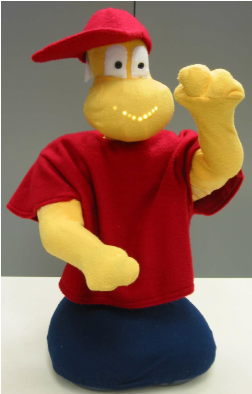
\includegraphics[width=1in]{images/Tito.png}
      \vspace{0.1cm}} & 
      \scriptsize{Creators: Audrey Duquette, François Michaud and Henri Mercier. Image: Assistive Technologies and Child-Robot Interaction – Scientific Figure on ResearchGate. Available from: \url{https://www.researchgate.net/Tito_fig2_249766819}}\\
      
     
      
      %Troy
      Troy & built for research with autistic children & pilot study \cite{giullian2010detailed}, long-term therapy \cite{goodrich2012incorporating}  & \parbox[c]{1em}{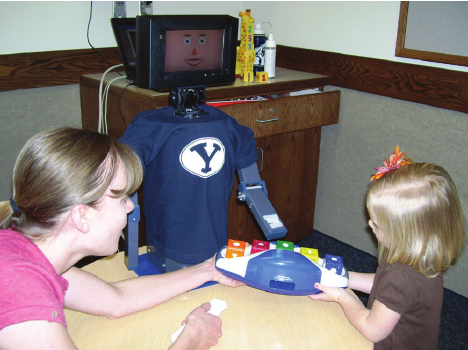
\includegraphics[width=1in]{images/Troy-BYUs-humanoid-robot.png}
      \vspace{0.1cm}} & 
      \scriptsize{Creators: J. Alan Atherton and Michael J. Goodrich. Image: Visual robot choreography for clinicians – Scientific Figure on ResearchGate. Available from: \url{https://www.researchgate.net/Troy-BYUs- humanoid-robot_fig1_224243058}}\\

      %Charlie
      Charlie  & built for research with autistic children & pilot study \cite{charlie2011}, interaction games \cite{boccanfuso2017low} & 
      \parbox[c]{1em}{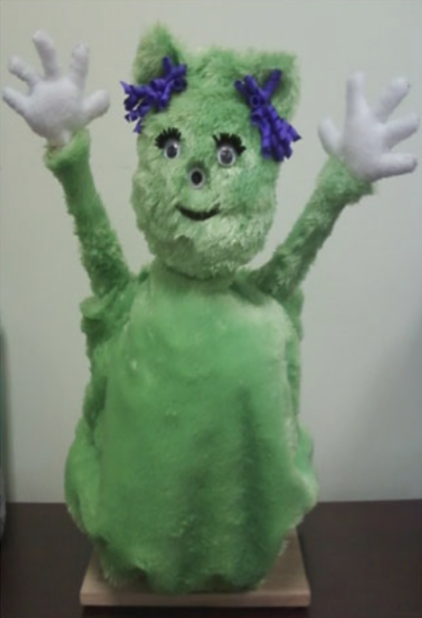
\includegraphics[width=1in]{images/charlie.png}\vspace{0.1cm}} & \scriptsize{Creators: Laura Boccanfuso and Jason M. O'Kane. Image: With kind permission from Springer Science + Business Media: Intl J Soc Rob, \cite{charlie2011}.} \\
      
      
      %built for research
      
      
      %Robota
      Robota  & built for research & long-term therapy \cite{robins2004effects}, effect of appearance of robot \cite{robins2006appearance} & \parbox[c]{1em}{      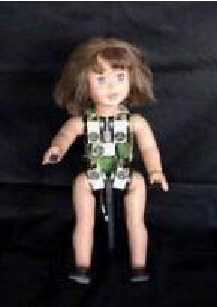
\includegraphics[width=1in]{images/Robota-Billard-et-al-2006.png}
      \vspace{0.1cm}} & 
      \scriptsize{Creators: Aude Billard at Adaptive Systems Laboratory at University of Lausanne. \cite{robotaRef}. Image: KASPAR – A Minimally Expressive Humanoid Robot for Human–Robot Interaction Research – Scientific Figure on ResearchGate. Available from: \url{https://www.researchgate.net/figure/Robota-Billard-et-al-2006_fig4_255601703}} \\
      
      
      %Keepon
      Keepon  & built for research & freeform interaction \cite{kozima2009keepon}  & \parbox[c]{1em}{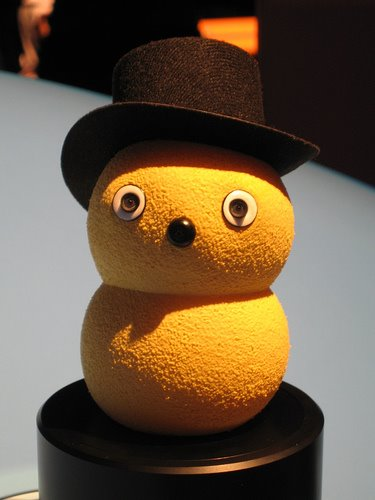
\includegraphics[width=1in]{images/KeeponTophatNextfest2007.jpg}
      \vspace{0.1cm}} & 
      \scriptsize{Creators: Hideki Kozima while at the National Institute of Information and Communications Technology. Image: Ilikedudes, from Wikimedia Commons.}\\
      
      
      %Probo
      Probo  & built for research & independent communicating during social stories \cite{pop2013social} & \parbox[c]{1em}{      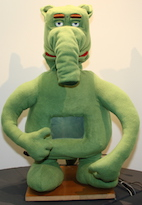
\includegraphics[width=1in]{images/probo.jpeg}\vspace{0.1cm}} & \scriptsize{Creators: Vrije Universiteit Brussel. Image: Probo, Vrije Universiteit Brussel \cite{ProboRef}.} \\
      
      
      %Kaspar
      Kaspar  & built for research  & interactive games \cite{wainer2014pilot}, co-creating autism interventions \cite{huijnen2017implement} & \parbox[c]{1em}{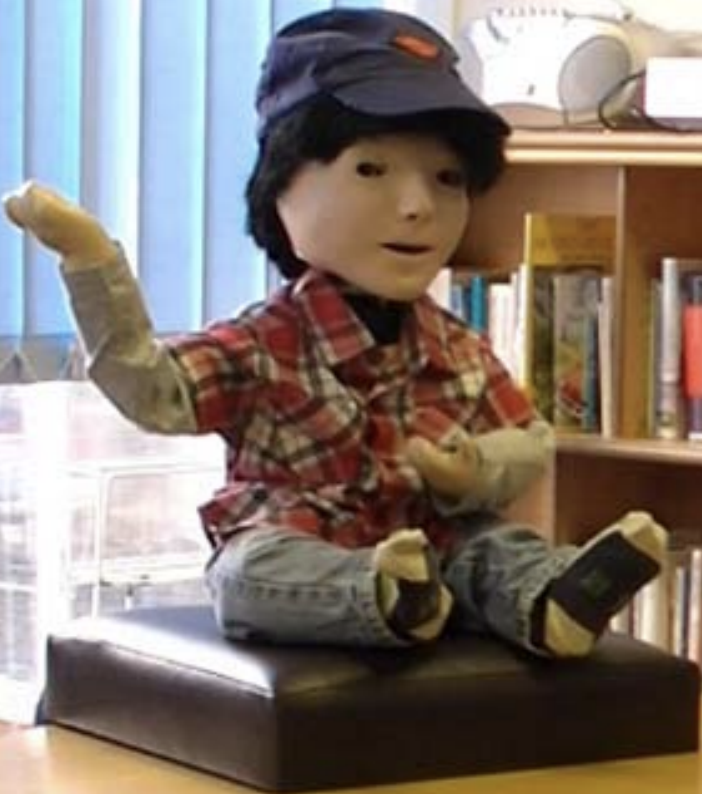
\includegraphics[width=1in]{images/kaspar.png}
      \vspace{0.1cm}} & 
      \scriptsize{Creators: Adaptive Systems Research Group at University of Hertfordshire \cite{kasparRef}. Image: Luke Wood, Kerstin Dautenhahn, A. Rainer, Ben Robins, Hagen Lehmann and Dag Sverre Syrdal. Used under a Creative Commons Attribution licence.}\\
      
      
      
      
      %built for commercial purposes
      
      %Nao
      Nao  & commercial, adapted for research & attention direction \cite{ARIA} & \parbox[c]{1em}{      \vspace{0.1cm}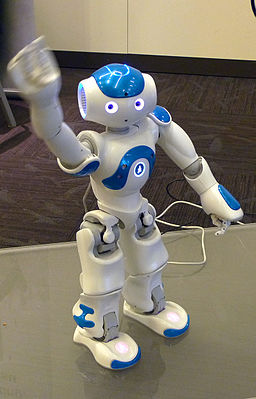
\includegraphics[width=1in]{images/NAO_waving.JPG}\vspace{0.1cm}} & \scriptsize{Creators: Aldebaran Robotics, acquired by Softbank Robotics \cite{NaoRef}. Image: Anonimski [CC0], from Wikimedia Commons.} \\
      
      
      %Pleo
      Pleo  & \vspace{0.1cm}commercial, adapted for research &robot as an embedded reinforcer of social behavior during semi-structured interactions \cite{kim2013social}, effect of positive affect during semi-structured interactions \cite{kim2015potential}\vspace{0.1cm}  & \parbox[c]{1em}{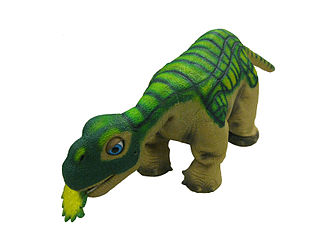
\includegraphics[width=1in]{images/Pleo_robot.jpg}\vspace{0.1cm}} & \scriptsize{Creators: Innvo Labs \cite{PleoRef}. Image: Jiuguang Wang, from Wikimedia Commons.}\\
      

      \hline
      
      
      \caption{Nine robots used in interventions targeting improvement of communication skills for children with ASDs. Pilot studies examining the robot's usability for this purpose, and studies where the robot was interacting with children with ASD are included. Robots are organized by category: robots that were designed specifically for use by children with autism first, robots that were designed for research and adapted for use by children with autism next, and robots that were designed for commercial use but adapted for research for children with autism last. Inside these categories, robots are organized according to oldest relevant research.}
      \label{table:robots}
    
  \end{longtable}


These nine robots are discussed in more detail below.


%autism robots
%Tito
\subsubsection{Tito}

Tito is a low-cost, custom-made robot for autism therapy created at the University of Sherbrooke. Tito is a small, cartoon-like robot that wears human clothes. 

Tito was used in an experiment to facilitate reciprocal interaction, such as imitative play. The experiment involved four low-functioning autistic children, two of whom interacted with the robot and two with a human mediator. The mediators executed imitation play patterns on three levels: facial expressions, body movements, and familiar actions with or without objects. Experiments were conducted with pre-programmed behaviors consisting of motion and vocal messages \cite{duquette2008exploring}.

The study measured shared focused attention and shared conventions, as well as absence of sharing, to determine the success of the interaction. The study showed that the robot mediator induced increased shared focused attention, visual contact and physical proximity, and children paired with it smiled more. However, children paired with the human mediator showed more shared conventions, such as imitation of body movements and familiar actions \cite{duquette2008exploring}.


%Troy
\subsubsection{Troy}

Troy was built at Brigham Young University for use in autism therapy. It is simple and mechanical in appearance, wears a human's shirt and pants, and has a screen as a face, on which different emotions can be displayed. Troy's behaviors were designed to encourage turn-taking and imitation in the child interacting with it \cite{goodrich2011case}.

The baseline of Troy in use for autism therapy was determined in a small study in 2010. The study showed that the robot could be controlled effectively during a therapy session, and that children seemed to treat it as a ``social other'' \cite{giullian2010detailed}.

In 2012, Troy was incorporated into an autism therapy team in longitudinal studies with two children with autism. The experimental set-up had a ``low-dose'' approach, where the robot was used for only 10 minutes during a 50 minute therapy session. The study noted increase in socially engaged behaviors as compared to before the study. The children also showed more interaction with the clinician after the treatment. Increase in greeting, symbolic play and sharing toys was also noted, as well as a decrease in restricted interests and repetitive behaviors \cite{goodrich2012incorporating}.


%Charlie
\subsubsection{Charlie}

Charlie is a low-cost robot, designed for use by children with autism in communication therapy, built at the University of South Carolina. The robot was explored in a pilot study in use with typically developing children in 2011. The robot taught imitation skills via the games ``Imitate Me, Imitate You'', and ``Pass the Pose''. Children interacted either only with the robot, imitating its movements and vice versa, or interacting with another child through the robot. The pilot succeeded as a proof-of-concept, as the neurotypical children interacted with the robot willingly, and it succeeded in operating as planned, detecting the children's faces and hands successfully \cite{charlie2011}.

At Yale university, Charlie was incorporated into an ASD-intervention within clinical methodology. The research noted improvements in communication and social interaction in the children, which were measured prior and after the interventions. The interventions focused on child-led interaction games \cite{boccanfuso2017low}.


%research robots
%Robota
\subsubsection{Robota}

Robota is a small, female-looking, doll-like robot, that was built at Adaptive Systems Laboratory at University of Lausanne \cite{billard2003robota}. Robota was designed to emphasize its humanoid aspect, and to have an especially human-like appearance for its face \cite{billard2006building}. 

Robota was not originally designed for use by children with autism, but has been applied as assistive technology in behavioral studies with low-functioning autistic children \cite{billard2006building}. Robota has been used in studies with autistic children by the AuRoRA research group, ``Autonomous Robot as a Remedial tool for Autistic children'', at the University of Hertfordshire \cite{robins2004effects, robins2006appearance}. AuRoRA is a research project initiated in 1988 at the University of Hertfordshire, studying the use of robots as tools that may serve an educational or therapeutic role for children with autism. Robota is autonomous, and has been taught sequences of actions and vocabulary using machine learning algorithms. Robota can react to touch by detecting passive motion of its limbs and head through its potentiometers \cite{robins2004effects}. 

AuRoRa used Robota to examine the long-term effects of use of a social robot in therapy with autistic children. This experiment was designed in response to the observation that one-time experiments are not likely to accurately predict what effects long-term therapy with robots could have. The change over time of eye gaze, touch and imitation in social interactions were observed. The experiment showed that all four children involved opened up socially to the robot and willingly interacted with it. The experiments also showed that conditions prior to arriving at the therapy, for example an unplanned change in schedule, which can be stressful for an autistic child, can significantly affect the child's behavior during the session \cite{robins2004effects}.

Robota was also used by AuRoRA to explore whether a robot's appearance matters in the interaction between an autistic child and the robot. The study showed that children with ASD have a preference for plain, featureless robots over robots with human-like features. The study compared Robota with a robotic appearance with a dressed-up, human-like Robota. Children displayed more social and pro-active behavior toward the plain Robota \cite{robins2006appearance}. Robota's appearance was subsequently changed to be more simple and robotic \cite{billard2006building}.


%Keepon
\subsubsection{Keepon}

Keepon is a small robot, designed for non-verbal, simple communication with children in order to study, test and elaborate on psychological models of development of social intelligence. It was designed by Hideki Kozima's research team at the National Institute of Information and Communications Technology in Kyoto. The minimalistic design has a yellow ``snowman''-like form, and was created after the same researchers determined that their toddler-sized and mechanical robot Infanoid provided too much stimulus for autistic children, and overwhelmed them so that they could not interact with it. Keepon has both an autonomous and teleoperated operation mode \cite{kozima2009keepon}.

Keepon has been used with both normally developing and autistic children. With autistic children, Keepon was observed to become regarded as a social actor by the children, increasingly toward the end of the their 15 interaction sessions over five months. The authors suggest that this indicates that autistic children do in fact have a motivation for sharing and exchanging mental states with others, contrary to popular belief (cf. \cite{carpenter2005role}). The researchers argue that when a robot is carefully designed to express its mental states in a way that is comprehensible to autistic children, they will establish a social relationship with it. Kozima argues that simple robots can facilitate exchange of mental states in children with autism, implying that the major social difficulties experienced by autistic children stem from difficulty of sifting out socially meaningful information in human interactions, rather than from lack of motivation \cite{kozima2009keepon}.


%Probo
\subsubsection{Probo}

The ``huggable robot'' Probo was designed at Vrije Universiteit Brussel, to be used by children in hospital contexts as a tele-interface for entertainment, communication and medical assistance. The social robot is a soft, elephant-like creature, with a screen in its stomach \cite{saldien2008design}. It has been adapted for research with autistic children.

An experiment conducted with 20 autistic children revealed that the children needed fewer communication prompts from the robot than a computer display, in order to respond to prompts given during a social story. The prompts were hierarchical, ranging from verbal to gestural and physical. The study examined the degree of independence of expressing social abilities such as asking questions, eye gaze, asking for help, and greeting. The use of Probo increased the independence of children expressing their social abilities \cite{pop2013social}.


%Kaspar
\subsubsection{Kaspar}

Kaspar, “Kinesics and Synchronization in Personal Assistant Robotics”, is a child-sized minimally expressive humanoid robot that has been developed by the Adaptive Systems Research Group at University of Hertfordshire. Kaspar is male-looking, has elastic skin and wears children's clothes. Kaspar was specifically designed to study human-robot interaction, with the aim of being able to signal emotions in a minimally expressive way \cite{dautenhahn2009kaspar}.

The AuRoRA research group has used Kaspar in several studies \cite{auroraProject}. Kaspar has been used to provide a predictable and repetitive experience of communication, which aims to be more comfortable for autistic children. Kaspar can be used to teach autistic children communication skills such as engaging in direct eye contact or taking turns. Kaspar also provides an enjoyable play context for the child to build their social skills \cite{kasparImpact}.

In the latest study by AuRoRA, Kaspar was used to explore the differences of a robot and a human playing partner in an interactive game with autistic children. The study concluded that children were more entertained by the robot, but more collaborative with human partners \cite{wainer2014pilot}.

Kaspar has also been used at other universities, such as Zuyd University of Applied Sciences, where it was used to co-create autism interventions together with autistic children, their parents and professionals of the field \cite{huijnen2017implement}. 


%commercial robots
%Nao
\subsubsection{Nao}

Nao is a commercial robot developed by Aldebaran Robotics in 2006, later acquired by Softbank Robotics \cite{NaoRef}. Nao is a small humanoid robot. It has been adapted as a research platform, due to its programmability.

In 2013, Nao was used as a tool to test robot-mediated joint attention skills with autistic children. The research involved creating a hierarchical structure of prompts executed by the robot to direct the child's attention. The study determined that children with autism showed a stronger preference toward robots over humans when compared to neurotypical children. Children with ASD also needed more prompts from the robot to successfully direct their attention than neurotypical children \cite{ARIA}.

The study concluded that using robots to teach social skills was promising, and they could be used to take advantage of autistic children's non-social attention preference. The study raised questions of how to generalize skills learned with the robot into everyday life \cite{ARIA}.


%Pleo
\subsubsection{Pleo}

Pleo is a small animatronic dinosaur toy, developed by Innvo Labs \cite{PleoRef}. Pleo has rudimentary sight, touch, temperature and motion sensors, and can understand basic voice commands.

The robot Pleo has been used to study the behavior of autistic children in semi-structured interactions \cite{kim2013social, kim2015potential}. Children were found to show more utterances toward an accompanying adult, when interacting with the robot in comparison to a computer screen \cite{kim2013social}. Researchers also noted more positive affect displayed by the child when interacting with the robot than with a human partner. Positive affect was defined as enjoyment or happy excitement. The study also noted that positive affect was related to greater autism severity, which meant that robots have the potential to be effective in interventions with lower functioning autistic individuals \cite{kim2015potential}.


%%%%%%%%%%
%%%%%%%%%%

\subsection{Sign language tutoring with social robots}

To my knowledge there is only one research group, the Cognitive Social Robotics Laboratory at Istanbul Technical University in Turkey, that has been studying robots as teachers of sign language to children \cite{CSRLpublications}. These studies have not researched the use of robots to teach sign language to children with ASD.



\subsubsection{Nao}

A study by the research group in 2011 explored the use of the Nao as a teacher of sign language for neurotypical children with normal hearing. In this study, non-verbal communication and imitation based interaction games between the robot and child were used to evaluate the children's ability to learn sign language from Nao \cite{taleofarobot}. Children readily imitated the robot during the study. The study referenced a previous study by the same research group, where the physical presence of a robot (Kaspar in particular) was determined to be more effective than a video of a robot \cite{kose2009effects}, and noted that this new study confirmed the result. The use of video as a sign language teaching method for children was not as effective as the use of a robot, because it lacks the social interaction dimension. The researchers also found that the effects of the physical limitations of the robots were diminished when the children had a relevant context or story for the signs \cite{taleofarobot}. 

This study did not research the use of the robot with children with ASD. The main observation from the study in the context of this thesis is that successful imitation of the robot by the human user can be used as a measure of successfully learning sign language from the robot.


\subsubsection{Robovie R3}

\begin{figure}
\centering
\urlstyle{same}
  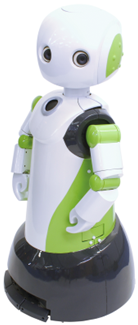
\includegraphics[width=1in]{images/robovieR3.png}
  \caption{Robovie R3. Creators: VStone \cite{Vstone}. Image: Advanced Telecommunications Research Institute International. Available at: \url{http://www.atr.jp/topics/press_100420_j.html}}
  \label{fig:robovie}
\end{figure}

A study done by the same research group in 2015 detailed how a five-fingered robotic platform, Robovie R3, was used to teach Turkish sign language to children. Robovie R3 is a humanoid robot with sophisticated hands, developed by Japanese company Vstone \cite{Vstone}. Robovie R3 is presented in figure \ref{fig:robovie}.

The study used imitation-based interaction games to tutor both children with hearing loss and children with normal hearing. The study aimed to establish interaction between the child and the humanoid robot through imitation and turn-taking. Robovie R3 was determined to be both successful in accurately demonstrating signs, and teaching the children \cite{uluer2015new}.

The study's robot was able to produce a set of 10 signs, chosen from a sub-set of daily used words. The same signs were used in the previous study with the robot Nao, and thus took into account Nao's physical limitations \cite{taleofarobot}. Due to its greater physical flexibility, Robovie R3 was determined to be a better sign language teacher than Nao \cite{uluer2015new}.

The robot was not examined in use by autistic children. The most important learning from this study in the context of this thesis is that imitation and turn-taking games were determined to be useful methodologies in a study examining whether users can learn sign language from a social robot.


\subsection{Design guidelines}

The robots discussed here, along with the observations and recommendations made in the studies, are used as a base to formulate design guidelines for a robot to be used to teach assistive signing to children with autism. In addition to this, explicit design recommendations and guidelines made by researchers for the design of social robots \cite{bartneck2004design}, and for robots specifically for use by autistic children \cite{designSpaces, giullian2010detailed, michaud2003characteristics, robins2007eliciting} are taken into account. Knowledge and research presented earlier in this chapter on how autism manifests and is treated in children is also applied to formulate the design guidelines.

The design guidelines will be used to guide the design process of the robot presented in this thesis, and will be utilized in the process of making explicit design decisions in the next chapter. While these guidelines have been developed with this particular application in mind, where the robot is used to teach assistive sign language to children with autism, these guidelines can be utilized in the design of robots for use by children with autism in general.

The design guidelines are:


\begin{itemize}

  \item \textbf{Simple form} \cite{charlie2011, boccanfuso2017low, designSpaces, duquette2008exploring, frith2003autism, giullian2010detailed, robins2007eliciting, robins2006appearance, kozima2009keepon}
  
  \item \textbf{Consistent, structured, simple behavior} \cite{bartneck2004design, charlie2011, boccanfuso2017low, billard2006building, designSpaces, duquette2008exploring, frith2003autism, giullian2010detailed, kim2013social, kim2015potential, kozima2009keepon, robins2007eliciting}
  
  \item \textbf{Positive, supportive, rewarding experience and environment} \cite{ARIA, charlie2011, boccanfuso2017low, carr1983acquisition, giullian2010detailed, huijnen2017implement, kim2015potential, kozima2009keepon, michaud2003characteristics, pop2013social, robins2004effects, robins2007eliciting, wainer2014pilot}
  
  \item \textbf{Modular complexity} \cite{ARIA, billard2006building, bonvillian1981sign, designSpaces, duquette2008exploring, giullian2010detailed, pop2013social, robins2007eliciting, robins2006appearance, tetzchner}
  
  \item \textbf{Modular specific to child's preferences} \cite{designSpaces, bonvillian1981sign, giullian2010detailed, robins2007eliciting, tetzchner}
  
\end{itemize}

The design guidelines are discussed in more detail below. Details on how the robots discussed in table \ref{table:robots} fulfill the design guidelines are presented in table \ref{table:guidelines}. The first three robots – Tito, Troy and Charlie – were designed specifically for use autistic children. Design guidelines are marked as fulfilled on the basis that a study conducted with the robot explicitly mentions the design condition being implemented or having pre-existed. Some robots that are introduced do exhibit realization of the design guidelines even if they are not explicitly mentioned. However, this is entirely up to the judgment of the observer, so these robots are not marked as following the design guidelines. For robots with multiple implementations across studies, if any implementation mentions the design guideline, they are included.


\begin{table}
 \bgroup
  \def\arraystretch{2}
  \centering
  \begin{tabular}{|p{2cm}|c|c|c|c|c|c|c|c|c|}
    \hline
     & 
    \scriptsize{Tito} &
    \scriptsize{Troy} &
    \scriptsize{Charlie} &
    \scriptsize{Robota} &
    \scriptsize{Keepon} &
    \scriptsize{Probo} &
    \scriptsize{Kaspar} &
    \scriptsize{Nao} &
    \scriptsize{Pleo} 
    \\\hline
    %\hline
    \scriptsize{Simple form} & x & x & x & x & x & – & – & – & – \\
    \scriptsize{Consistent, structured, simple behavior} & x & x & x & x & x & – & – & – & x \\
    \scriptsize{Positive, supportive, rewarding experience and environment} & – & x & x & x & x & x & x & x & x \\
    \scriptsize{Modular complexity} & x & x & – & x & – & x & x & x & –  \\
    \scriptsize{Modular specific to child's preferences} & – & – & – & – & – & – & / & – & – \\
     \hline
  \end{tabular}
  \caption{This table details how the robots presented in table \ref{table:robots} follow the established design guidelines in their relevant studies. If the robot follows a design guideline, it is marked with an ``x'', if they do not, it is marked with a ``–''. The ``/'' indicates that this is an emerging realization of a design guideline.}
  \label{table:guidelines}
  \egroup
\end{table}


\subsubsection{Simple form}

As discussed previously in this chapter, people with autism have problems with forming a holistic perception, meaning they have problems integrating different stimuli into a ``wholesome'' experience, and may instead fixate on isolated features \cite{designSpaces, frith2003autism, giullian2010detailed}. To avoid overstimulation, social robots designed for use by autistic children should be kept simple and predictable in their appearance \cite{designSpaces, kozima2009keepon, robins2007eliciting}. Additionally, an appearance that is too life-like and close to a human could even unnecessarily limit the robot and restrict its functionalities \cite{designSpaces}.

Robots examined in table \ref{table:robots} which have been designed specifically for use by autistic children have all been kept simple in form and appearance, as seen in table \ref{table:guidelines}. The robot Charlie was created to have simple, toy-like and friendly appearance to more easily attract the attention of a child, and to appear approachable and not intimidating \cite{charlie2011, boccanfuso2017low}. The robot Tito was described by researchers to be simple and human-like in appearance \cite{duquette2008exploring}. The robot Troy was designed to not be overly realistic, and to have a simple and mascot-like appearance. It was designed to have a mechanical appearance in order to be discernable as a robot, but not too mechanical so that the child would not become fixated on its components. The robot's face, which is a computer screen, has a cartoonish and simple design \cite{giullian2010detailed}.

Robota, a robot applied to behavioral studies with autistic children, was especially designed to be humanoid in appearance \cite{billard2006building}. However, it was later discovered in a study with Robota that children preferred it to have a simpler, robotic appearance \cite{robins2006appearance}. The appearance was changed accordingly for subsequent use by children with autism \cite{billard2006building}.

The robot Keepon, which was designed for interaction with children, was also designed to be simple in appearance, and to have basic anthropomorphic traits such as lateral symmetry and two eyes, to indicate potential for social agency. The designers also opted to convey Keepon's emotions through bodily movement, avoiding facial expression in order to not risk a flood of information \cite{kozima2009keepon}.


\subsubsection{Consistent, structured, simple behavior}

As discussed, people with autism have problems with social interaction and flexibility of behavior and routines \cite{frith2003autism, tetzchner}. Their lack of Theory of Mind leads them to be unable to predict other people's behavior \cite{baron1985does, frith2003autism}. Robots that behave consistently and predictably could potentially bridge the gap for autists confused by human complexity, and help them learn communication skills \cite{designSpaces, robins2007eliciting}. A large number of features in behavior could even be overwhelming \cite{designSpaces}, and result in overstimulation \cite{designSpaces, kozima2009keepon}. A consistent set of behaviors \cite{bartneck2004design}, as well as a structured sequence of actions and positive behavior reinforcement is recommended \cite{robins2007eliciting}.

All robots examined in table \ref{table:robots}, which have been designed for children with autism, follow this design guideline (as seen in table \ref{table:guidelines}). The robot Tito was described by researchers to be more predictable than humans \cite{duquette2008exploring}. Troy's behavior was designed to be simple and clearly structured through if/else branching and do/while loops. Some adaptability was built in, so that a therapist could make changes during a therapy session \cite{giullian2010detailed}. The games that the robot Charlie was designed to play with children, ``Imitate Me, Imitate You'' and ``Pass the Pose'', both follow a consistent and structured behavioral flow \cite{charlie2011}. The same simple games were further developed in a later study with Charlie \cite{boccanfuso2017low}.

Robota can engage in both simple and complex behaviors with the user, depending whether it is performing its ``built-in'' or ``learning'' behaviors. Robota's simple behaviors include simple imitation of the user, and simple expression of emotions \cite{billard2006building}.

Keepon's behavior was kept simple and constituted of two actions: attentive orienting toward a certain target by directing its head toward it, and emotive expression by rocking its body up and down. These behaviors aimed to communicate what Keepon perceives, and how it evaluates the target \cite{kozima2009keepon}.

Pleo was pre-programmed with 13 socially expressive behaviors \cite{kim2013social}. In a later study, its behavior was constrained to a pre-determined set, which were delivered according to a tightly controlled interactive script \cite{kim2015potential}.



\subsubsection{Positive, supportive, rewarding experience and environment}

Learning a new method of communication requires the co-operation and support of the child's speech therapist, loved ones and other educators they may have \cite{tetzchner}. Involving the people present in the child's everyday life, and practicing in familiar environments, can help aid generalization and creates a supportive experience \cite{carr1983acquisition}. An encouraging and supportive environment congratulates the child when they are doing well, but is not too critical if the child should respond incorrectly \cite{michaud2003characteristics, robins2007eliciting}. A sensory reward for participating in the therapy is recommended to keep the child motivated and the experience positive \cite{ michaud2003characteristics, robins2007eliciting}. The robot should be a companion to the child, and be receptive and responsive to the child's actions \cite{robins2007eliciting}. Eight out of the nine examined robots follow this design guideline, as seen in table \ref{table:guidelines}.

Troy is designed to involve the therapist of the child in a triadic interaction with the robot, with the robot acting as a facilitator of social interaction, in order to aid generalization. Troy is responsive to the child's behavior \cite{giullian2010detailed}.

Charlie was designed to provide positive sensory feedback, in the form of LEDs flashing in its hands, when the child successfully imitated the robot's pose. The robot could also provide positive auditory feedback. If the child did not respond, the robot did not criticize the child, but continued with the game \cite{charlie2011, boccanfuso2017low}. 

Robota was used in a reassuring environment, where the robot's predictability and repetitive behavior were comforting factors \cite{robins2004effects}. Keepon was situated in the naturalistic environment of the children's preschool playroom, in order to create a supportive environment \cite{kozima2009keepon}. Probo was designed to offer positive feedback to the user when they answered correctly in order to reward them, and to correct wrong answers \cite{pop2013social}.

In a co-creation study, positively reinforcing behaviors, such as rewarding, were designed for Kaspar. Participants suggested that Kaspar could give a thumbs up to reward the chidlren in a non-verbal manner.  If the child made a mistake, Kaspar was designed to give a reaction in a neutral voice, without an angry tone \cite{huijnen2017implement}. In another study, sensory rewards were designed to be used in the experiment environment, when the child behaved correctly. Rewards were implemented either as visuals on a separate screen, or as a reward sound. Children seemed to enjoy the sensory rewards. Additionally, the study concluded that the interaction with Kaspar had been a positive experience, as children displayed positive affect, such as smiling when interacting with the robot \cite{wainer2014pilot}.

The robot Nao was used to generate sensory rewards and encouragement to autistic children who responded correctly to attention prompts. The robot would for example say ``Good job!'', and a movie clip would play on a screen. When the children responded incorrectly, the robot issued the next level of prompt \cite{ARIA}.

The robot Pleo was used to study the role of positive affect on communication and social skills during interventions with autistic children. The robot was designed to maintain a child's engagement through positive affect \cite{kim2015potential}.


\subsubsection{Modular complexity}

Due to the level of functioning among individuals with ASD being highly variable \cite{WHOautism}, the individual's social and cognitive skills and needs should be taken into account when designing the complexity of the robot \cite{bonvillian1981sign, designSpaces, tetzchner}. In the initial design of the robot, the first two design guidelines, ``simplicity of form'' and ``consistent, structured, simple behavior'' should be followed. However, as the child's skills develop, the robot's qualities, including form and behavior, should become increasingly complex, in order to continue challenging and teaching the child. Six out of the presented robots follow this design guideline (table \ref{table:guidelines}).

The complexity of the robot's behavior needs to be structured so that the child knows what to expect, but also evolve continually to keep the child's interest \cite{designSpaces, michaud2003characteristics}. Interaction complexity should also be modular. Built-in capacity to gradually increase complexity of interaction, to promote further learning is recommended \cite{designSpaces, robins2007eliciting}. This can be done through developing different interaction modalities, such as using lights and sounds \cite{robins2007eliciting}. Complexity of the robot's appearance could also be increased over time \cite{robins2007eliciting}, for example by making it appear more human-like with clothing or wigs.

The robot Tito was studied as a social mediator, where three levels of imitation were organized in increasing complexity, varying the interaction complexity \cite{duquette2008exploring}.

Modularity of complexity has been previously used in a comparative behavioral study with the Nao robot, where hierarchical communication prompts were made by the robot to the child \cite{ARIA}. Hierarchical prompting was also used in a study comparing the robot Probo with a computer display \cite{pop2013social}. Both studies showed that different children needed different complexity levels of prompting to respond. 

Modularity of complexity was built-in into the design of Troy. Its face, which is a screen, has a simple cartoonish face initially, but could eventually show the image of a human's face to achieve increased realism. This is designed with the goal to aid generalization of skills learned with the robot \cite{giullian2010detailed}. For Troy's behavior, sub-choreographies of behavior were designed to be chosen based on the particular child who the therapist would be treating. If one of the sub-choreographies did not elicit desired behavior from the child, the therapist could change what the robot was doing \cite{giullian2010detailed}.

Robota can engage in increasingly complex behaviors with its user while in ``learning'' mode. The user can for example teach the robot to dance or teach it a simple vocabulary \cite{billard2006building}.

One of the co-created interventions for Kaspar details the level of intervention increasing and decreasing according to the child, in order to ensure generalization \cite{huijnen2017implement}.


\subsubsection{Modular specific to child's preferences}

Modularity specific to a child's preferences can be thought to include the previously mentioned modularity of complexity, which takes into account the child's pre-existing social and cognitive skills. However, here the distinction is made that this design guideline targets modularity that incorporates a child's interests or needs in another way. In communication therapy interventions for autism, the individual's needs and interests need to be taken into account \cite{bonvillian1981sign, tetzchner}. As autism is a spectrum, designing one static robot to fit all autistic children's needs is not possible. Built-in modularity of the robot's behavior, form, and other qualities is useful for this reason \cite{designSpaces,robins2007eliciting}.

The robot's actions should adapt to the child's responses and their level of interest \cite{giullian2010detailed}. The robot should be modifiable for different therapeutic solutions, including different interaction modalities and interaction scenarios \cite{designSpaces, robins2007eliciting, michaud2003characteristics}. Children's personal interests can be used to modify interactions \cite{designSpaces, robins2007eliciting}, for example by discussing the child's interests during the therapy, or incorporating music that the child likes into the therapy. For children prone to overstimulation, for example by flashing lights, any lights on the robot should be disabled. The robot should be adaptable to a personalized and familiar context or environment, such as the child's home, so it can be explored in a safe setting \cite{robins2007eliciting}.

Modularity specific to a child's preferences (excluding modularity of complexity) has not been studied in robotic interventions to my knowledge. This could be due to the fact that robotic interventions have not yet reached the level of sophistication to implement child-specific requirements, and are instead in the pilot levels of study.

The robot Troy's designers mention adapting the robot's behavior's complexity according to how the child responds in therapy \cite{giullian2010detailed}. However, this does not respond to the child's specific interests or preferences, rather their level of learning. Similarly, an intervention implemented with the robot Kaspar details increasing or decreasing the level of intervention according to the child \cite{huijnen2017implement}. This is not responding to the child's preferences, but rather their level of learning, and in fact follows the ``modular complexity'' design guideline, rather than the ``modular specific to child's preferences'' guideline.

However, a ``girl-version'' of the robot Kaspar, Kassy, was created in response to co-creation studies with professionals of autism interventions recommending it \cite{huijnen2017implement}. This gender-specific design modification can be seen as a step in the direction of designing robots specific to children's personal preferences. The emerging realization of this design guideline is given acknowledgement in the table \ref{table:guidelines}.


\section{Summary}

In this chapter, research on autistic children, their difficulties communicating, and sign language as a communication method is reviewed. Additionally, research on social robots that have previously been used to perform communication therapy with autistic children is reviewed. Insights from this research have been synthesized to form design guidelines.

In the next chapter, the design guidelines will be used to guide the design decisions made to create a robot for the purpose of teaching assistive signs to children with ASD. The design guidelines fit into a design framework for social robots.

The five design guidelines defined in this chapter can be used to guide the design of robots for use by children with autism in general. 

The other key outcome of this literature review is insight from previous studies on teaching sign language with robots to neurotypical children. This informs the design of the experiment described in chapter \ref{chapter:methods}. 
